\documentclass[12pt]{article}
\usepackage[polish]{babel} 
\usepackage[T1]{fontenc} % obsługa polskich znaki
\usepackage[utf8]{inputenc} % użycie kodowania UTF-8 dla pliku źródłowego
\usepackage{enumitem} % dodatkowe narzędzie do konfiguracji list
\usepackage{comment} % Import pakietu comment

\usepackage{amsmath}
\usepackage{amsfonts}
\usepackage{amssymb}
\usepackage{amsthm}
\usepackage{makeidx}
\usepackage{graphicx}
\usepackage{float}  % Dołącz w preambule
\usepackage{array}  % Załaduj pakiet array dla zaawansowanych funkcji tabel

\DeclareUnicodeCharacter{00B3}{\textsuperscript{3}}

\usepackage{pgfplots}
\pgfplotsset{compat=1.17}


\usepackage{listings}
\usepackage{color}

\lstset{frame=tb,
  language=Java,
  aboveskip=3mm,
  belowskip=3mm,
  showstringspaces=false,
  columns=flexible,
  basicstyle={\small\ttfamily},
  numbers=none,
  numberstyle=\tiny\color{gray},
  keywordstyle=\color{blue},
  commentstyle=\color{dkgreen},
  stringstyle=\color{mauve},
  breaklines=true,
  breakatwhitespace=true,
  tabsize=3
}

\definecolor{dkgreen}{rgb}{0,0.6,0}
\definecolor{gray}{rgb}{0.5,0.5,0.5}
\definecolor{mauve}{rgb}{0.58,0,0.82}

\usepackage{multicol}

\title{Algorytm szybkiej odwrotności pierwiastka kwadratowego przez stałą szesnastkową $0x5f3759df$ z 32-bitowej liczby zmiennoprzecinkowej w standardzie IEEE 754.}
\author{Bartosz P. Szczepaniok}
\date{20 kwietnia 2024}

\begin{document}

\maketitle

\begin{abstract}
\noindent Algorytm szybkiej odwrotności pierwiastka kwadratowego, zastosowany w Quake III Arena, zapewnia efektywną normalizację wektorów w przestrzeni trójwymiarowej, co było kluczowe dla wydajności w grafice komputerowej i fizyce gier.  Artykuł omawia historie i szczegółowo wyjaśnia działanie algorytmu, jego problematykę w implementacji w języku wysokopoziomowych oraz to dla jakich dziedzin techniki i informatyki miał zastosowanie.
\end{abstract}

\section{Wprowadzenie}
Terje Mathisen, programista w firmie id Software w roku 1999 stanął przed pewnym problem. Problem, z którym się mierzył, dotyczył efektywności i szybkości obliczania odwrotności pierwiastka kwadratowego liczb zmiennoprzecinkowych, co było potrzebne przy normalizacji wektorów. Przede wszystkim, dlaczego silnik gry miałby obliczać $1/sqrt(x)$? Jeśli program ma mieć zaimplementowaną fizykę, oświetlenie lub odbicia światła w swoim silniku gry, warto używać znormalizowanych wektorów o długości 1. W przeciwnym razie wektory mogą być zbyt krótkie lub zbyt długie, co może prowadzić do błędów w obliczeniach. 

\noindent Długość wektora w przestrzeni trójwymiarowej oznaczamy następująco:
$$ \begin{cases}
|\mathbf{a}| = \sqrt{x_a^2 + y_a^2 + z_a^2}
\end{cases} $$

\noindent Aby znormalizować wektor, trzeba przeskalować jego wartość do długości 1. Otrzymujemy to dzieląc długość wektora przez długość wektora. 
$$ \begin{cases}
\frac{\sqrt{x^2 + y^2 + z^2}}{\sqrt{x^2 + y^2 + z^2}} = 1
\end{cases} $$

\noindent W skutek czego każdy z jego składników należy podzielić przez jego długość. 
$$ \begin{cases}
\frac{x}{\sqrt{x^2 + y^2 + z^2}}
\frac{y}{\sqrt{x^2 + y^2 + z^2}}
\frac{z}{\sqrt{x^2 + y^2 + z^2}}
\end{cases} $$

\noindent Obliczanie $x^2 + y^2 + z^2$ jest dość łatwe a co ważniejsze szybkie. Problem polega na tym, że operacje pierwiastkowania i dzielenia nie są najszybsze.  Dla tysięcy powierzchni w grze, z których każda ma wektor do znormalizowania, staje się to problemem. Stąd, szybka odwrotność pierwiastka kwadratowego jest kluczowa, zapewniając trzy razy szybsze obliczenia przy błędzie nie większym niż 1 procent.

\section{Metody}

\subsection{Algorytm}

\begin{lstlisting}
float Q_rsqrt( float number )
{
    long i;
    float x2, y;
    const float threehalfs = 1.5F;

    x2 = number * 0.5F;
    y  = number;
    i  = * ( long * ) &y;     // evil floating point bit level hacking
    i  = 0x5f3759df - ( i >> 1 );              // what the fuck?
    y  = * ( float * ) &i;
    y  = y * ( threehalfs - ( x2 * y * y ) );  // 1st iteration
//	y  = y * ( threehalfs - ( x2 * y * y ) );  
// 2nd iteration, this can be removed

	return y;
}
\end{lstlisting}

\noindent Na początku kod wydaje się dość prosty. Funkcja przyjmuje liczbę, która ma być obliczona, jako wejście.

\begin{lstlisting}
float Q_rsqrt( float number )
{
    long i;                        // 32-bitowa liczba całkowita
    float x2, y;                   // 32-bitowa liczba dziesiętna
    const float threehalfs = 1.5F; //1.5 również jako liczba 32 bitowa

\end{lstlisting}

 \noindent Zmienna $i$ jest deklarowana jako 32-bitowa liczba całkowita. Następnie $x2$ i $y$ to 32-bitowe liczby dziesiętne, zapisujemy wartość $1,5$ do zmiennej o nazwie $threehalfs$. 

 \begin{lstlisting}
float Q_rsqrt( float number )
{
    x2 = number * 0.5F;
    y  = number;
 

\end{lstlisting}
 	
 
\noindent Następne dwie linie kodu kopiują połowę inputu do $x2$, a całość do $y$. 

\subsection{Struktura bitowa liczby}

\noindent Aby zrozumieć algorytm, musimy przyjrzeć się binarnym reprezentacjom liczb. W języku C deklarujemy 32-bitową liczbę całkowitą jako long. Problem pojawia się w kolejnym kroku gdzie mamy dwie liczby dziesiętne. Wykorzystujemy standard IEEE 754, który opisuje, jak te liczby są kodowane. Standard ten wykorzystuje zapis notacji naukowej.

Pierwszy bit odpowiedzialny jest za znak, algorytm w quakeu przyjmował tylko wartości dodatnie więc w tym wypadku zawszę będzie wynosił 0. 

Kolejne 8 bitów wyrażają wykładnik liczby 2, pozwala nam to na wyznacznik z zakresu <255, 0>, jednak z racji tego że chcemy liczyć wykładnik ujemny dlatego zakres zmniejszamy o 127 uzyskując zakres <128, -127>. Tak więc dla wykładnika równego 4 wartość bitowa musi wynosić 131 (ponieważ 131 - 127 daje nam wartość 4).

Ostatnie 23 bity odpowiadają to mantysie w postaci wykładniczej. 

\begin{table}[htbp]
\centering
\caption{Reprezentacja binarna liczby zmiennoprzecinkowej}
\label{tab:struktura bitowa floata}
\begin{tabular}{|c|c|c|}  % 'c' oznacza wyśrodkowaną kolumnę, '|' oznacza linie pionowe
\hline  % Dodaje poziomą linię na górze tabeli
Bit znaku (s) & Wykładnik (E) & Mantysa (M) \\ \hline  % Pierwszy wiersz danych
31 bit & 30 - bity - 23 & 23 - bity - 0 \\ \hline  % Drugi wiersz danych
\end{tabular}
\end{table}

\noindent Należy przyjąć myślenie o mantysie i wykładniku jako o binarnych liczbach, które nimi są. Jeśli mamy dwie liczby, jedna będąca mantysą $(M)$, a druga wykładnikiem $(E)$ otrzymujemy, odpowiednio 23 bity i 8 bitów:

\begin{lstlisting}
    M                                  0000 0000 0000 0000 0000 000
    E                                                       0000 0000
\end{lstlisting}

\noindent Tak więc tak można zapisać bity, ale faktyczną liczbę za tymi bitami otrzymujemy z tego wzoru

$$ \begin{cases}
(1 + \frac{M}{2^{23}}) * 2^{E-127}
\end{cases} $$

\noindent To forma powinna wyglądać znajomo, wzór składa się z wykładnika (E) pomniejszony o 127 wraz mamy mantysę (M) z dodatkową jedynką (s - determinuje liczbe jako dodatnią) na początku, dokonujemy teraz przekształcenia wkładając nasz wzór do logarytmu o podstawie 2.

$$ \begin{cases}
log_2((1 + \frac{M}{2^{23}}) * 2^{E-127})
\end{cases} $$

$$ \begin{cases}
log_2(1 + \frac{M}{2^{23})} + log_2(2^{E-127})
\end{cases} $$

$$ \begin{cases}
log_2(1 + \frac{M}{2^{23}}) + E-127
\end{cases} $$

\noindent Jest to najbardziej uproszczona forma wzoru, należy teraz skorzystać z właściwości aproksymacji logarytmu:

$$ \begin{cases}
log2(1 + x) \approx x
\end{cases} $$

\noindent Dla małych wartości $x$, $log_2(1+x)$ w przybliżeniu wynosi $x$. Poniższy wykres pokazuje że dla wartości $0$ oraz $1$ funkcje na siebie nachodzą. 

\begin{figure}[H]  
\centering
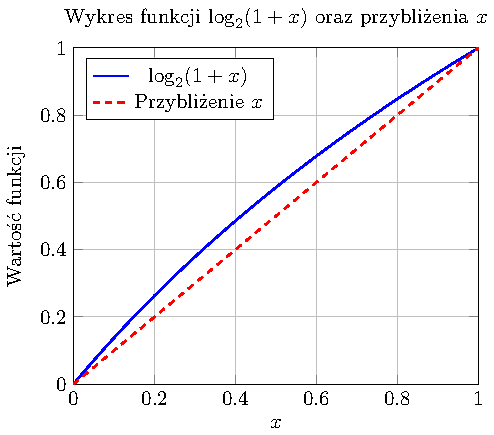
\includegraphics[width=0.5\textwidth]{aproksymacja.pdf} 
\caption{Porównanie funkcji $\log_2(1 + x)$ i jej przybliżenia $x$.}
\label{fig:log_approx}
\end{figure}

\noindent Do całości należy dodać następujący termin $\mu$, będzie to różnica wartości między $x$ a jego przybliżeniem. Dla wartości $\mu$ równej 0.043 dostajemy najmniejszy błąd dla średniej

\begin{figure}[H]  
\centering
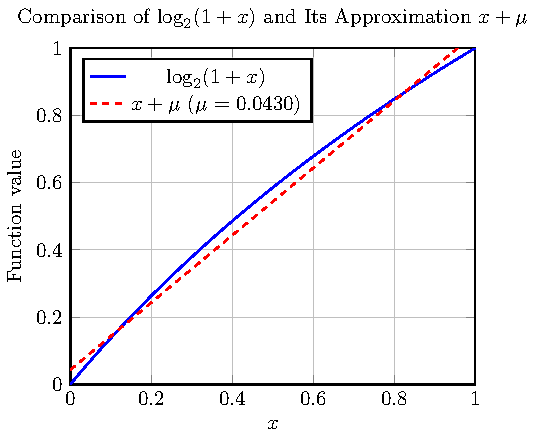
\includegraphics[width=0.5\textwidth]{aproksymacja_mu.pdf} 
\caption{Porównanie funkcji $\log_2(1 + x)$ i jej przybliżenia $x$. ze zmienną $\mu$}
\label{fig:log_approx}
\end{figure}

\noindent Wracając do wzoru, podstawmy aproksymacje dla którego otrzymujemy:

$$ \begin{cases}
\frac{M}{2^{23}} + \mu + E-127
\end{cases} $$

\noindent Po kolejnych uproszczeniach dochodzimy do: 

$$ \begin{cases}
\frac{M}{2^{23}} + \frac{2^{23}*E}{2^{23}} + \mu - 127
\end{cases} $$

$$ \begin{cases}
\frac{1  (M + 2^{23} * E)}{2^{23}} + \mu + -127
\end{cases} $$

$$ \begin{cases}
\frac{1}{2^{23}}  (M + 2^{23} * E) + \mu + -127
\end{cases} $$

\noindent $(M + 2^{23} * E$ pojawiło się wcześniej jako reprezentacja binarna. Resumując aplikując logarytm o podstawie z dwóch do naszego wzoru otrzymujemy reprezentacje bitową naszej naszej liczby przekształconą przez stałe, w pewnym sensie reprezentacja bitowa liczby jest swoim własnym logarytmem. Z tą wiedzą możemy nareszcie przejść do właściwego algorytmu.

\subsection{Evil floating point}

\begin{lstlisting}
    i  = * ( long * ) &y;     // evil floating point bit level hacking
\end{lstlisting}

Mamy tu do czynieniem z manipulacją adresem pamięci. Po przypisaniu naszej liczby po zmienną y chcemy dokonać pewnych manipulacji na jej bitach. Format float nie pozwala na manipulacje bitami, w przeciwieństwie do typu long.

\begin{lstlisting}
    i  = ( long ) y;     
\end{lstlisting}

C jak większość języków programowania pozwala na przypisywanie zmiennej innego typu. Taka konwersja z liczby całkowitej na zmienno-przecinkową mocno miesza zapis bitowy. 3.33 użyte w przykładzie ma nasz zapis binarny (bit znaku, wykładnik oraz mantysa) natomiast 3 to zapis zwykły zapis binary

\begin{lstlisting}
        3.33        -> 0 10000000 10101010001111010111000
        3           -> 00000000 00000000 00000000 00000011
\end{lstlisting}


\noindent To co chcemy osiągnąć to bez zmian na bitach zapisać longa w typie float. Żeby to osiągnąć trzeba zmienić miejsce w pamięci, a nie samą liczbę. Pobierając adres zmiennej y przypisujemy go pod adres zmiennej long (i). Sam adres pozostaje taki sam, natomiast kompilator uważa że liczba pod tym adresem jest longiem. 

\subsection{Magiczna liczba}

\begin{lstlisting}
    i  = 0x5f3759df - ( i >> 1 );   
\end{lstlisting}

Operacja bitowa w tym miejscu zmniejsza nam liczbę dwukrotnie. Dla wykładnika oznacza to:

$$ \begin{cases}
x >> x^{\frac{1}{2}}
\end{cases} $$

\noindent Połączenie z negacja wykładnika daje nam to czego od początku szukamy czyli $1/sqrt(x)$
\newline
\newline

Wracając do głównego problemu którym jest wydajność takich operacji jak pierwiastkowanie i dzielenie, wykazaliśmy że że z równania $1/sqrt(x)$ zapisując pod zmienną $i$ wartość bitową zmiennej $y$ możemy zapisać jako:

$$ \begin{cases}
\frac{1}{\sqrt{y}} = \log\frac{1}{\sqrt{y}} = \log(y^{-\frac{1}{2}}) = -\frac{1}{2}\log(y)
\end{cases} $$

\noindent Z tej formy znacznie łatwiej i szybciej policzyć pierwotne wyrażnie, tym bardziej że teraz wiemy czym jest manipulacja bitowa. Zamiast dzielić cały logarytm przez $-\frac{1}{2}$ dokonujemy właśnie tą operacje $-(i >> 1)$
\newline

Ale dlaczego pojawia się tutaj stała szesnastkowa? Ponieważ nasz logarytm jest przeskalowany i bitowo przesunięty. Niech Gamma będzie rozwiązaniem naszego równania. Dokonajmy znów prostych przekształceń

$$ \begin{cases}
\Gamma = \frac{1}{\sqrt{y}}
\end{cases} $$

$$ \begin{cases}
\log(\Gamma) = \log(\frac{1}{\sqrt{y}})
\end{cases} $$

$$ \begin{cases}
\log(\Gamma) = -\frac{1}{2}\log(y)
\end{cases} $$

\newpage
\noindent Teraz podstawiamy pod logarytm nasz wzór opisujący reprezentacje bitową.

$$ \begin{cases}
\frac{1}{2^{23}}(M_{\Gamma} + 2^{23} * E_{\Gamma}) + \mu - 127 = -\frac{1}{2}(\frac{1}{2^{23}}(M_y + 2^{23} * E_y) + \mu - 127)
\end{cases} $$

$$ \begin{cases}
(M_{\Gamma} + 2^{23} * E_{\Gamma}) = \frac{3}{2}2^{23}(127 - \mu)-\frac{1}{2}(M_y + 2^{23} * E_y)
\end{cases} $$

\noindent Nasza liczba szesnastkowa $0x5f3759df$ okazuje się być pozostałości: błędu $\mu$, współczynniku skalowania i przesunięcia naszej liczby $y$
\newline
\begin{lstlisting}
    y  = * ( float * ) &i;     
\end{lstlisting}

Następnym krokiem algorytmu przypisanie adresu i który już przeskalowany i przesunięty da nam przybliżenie wartości x której szukamy już w formie liczby zmiennoprzecinkowej a nie wartości bitowej. Jest to krok odwrotny do wcześniejszego.

\subsection{Iteracja Newtona-Raphsona}

Po poprzednim kroku mamy dość przyzwoite przybliżenie naszego wyrażenia ale wychwyciliśmy tutaj pewne błędny bo liczyliśmy przybliżenie zamiast całkowitego wyrażanie, ale dzięki metodzie Newtona możemy dojść do naprawdę dobrego przybliżenie zamiast na przyzwoitym.
\newline

Metoda Newtona jest techniką, która znajduje pierwiastek dla danej funkcji co oznacza, że znajduje $\sqrt{x}$, dla którego $f(x) = 0$.

\hfill \break
Dzieje się tak bo metoda Newtona bierze przybliżenie a następnie zwraca bardziej dokładne przybliżenie do momentu wyznaczenia odpowiednio dokładnego przybliżenia. W praktyce w opisywanym przezemnie algorytmie już jedna iteracja metodą Newtona pozwala na przybliżenie o błędzie 1 procenta.

Jedyne czego ta iteracja potrzebuje, to funkcje i jej pochodną. Robi to przyjmując wartość $x$ i próbując zgadnąć, o ile jest $x$ jest różny od bycia pierwiastkiem, a robi to poprzez obliczenie $f(x)$ i jego pochodnej $f'(x)$

\newpage
\noindent Może naszą wartość $f(x)$ zapisać jako $\Delta{y}$ a naszą pochodną  $f'(x)$ jako $\frac{\Delta{y} }{\Delta{x} }$ naszą zmianą odległości między $x$ a szukaną wartością $\sqrt{x}$ oznaczmy jako $\Delta{x}$

$$ \begin{cases}
\frac{\Delta{y} }{\Delta{x} } * \Delta{x} = \Delta{y}
\end{cases} $$

$$ \begin{cases}
\Delta{x} = \frac{\Delta{y}}{\frac{\Delta{y} }{\Delta{x} }} \implies \frac{f(x)}{f'(x)}
\end{cases} $$

$$ \begin{cases}
x_{root} = x -\frac{f(x)}{f'(x)} 
\end{cases} $$

\noindent I w ten sposób aby wyznaczyć nową, bardziej przybliżoną wartość x, należy odjąć od x iloraz funkcji przez jej pochodną

\begin{lstlisting}
   y  = y * ( threehalfs - ( x2 * y * y ) );  // 1st iteration
//	y  = y * ( threehalfs - ( x2 * y * y ) );  
// 2nd iteration, this can be removed
\end{lstlisting}

Ostatnia linijka kodu jest właśnie iteracją Newtonowską zastosowaną do funkcji $f(x) = \frac{1}{y^2} - x$. Należy zwrócić uwagę że dla y będącego pierwiastkiem tej funkcji jest równoważna dla y będącemu odwrotnością kwadratu pierwiastka x:

$$ \begin{cases}
f(x) = 0 \implies 0 = \frac{1}{y^2} - x \implies x = \frac{1}{y^2} \implies y = \frac{1}{\sqrt{x}}
\end{cases} $$

\section{Materiały}
Po poprzednim akapicie nasuwa się pytanie, czy nie możemy użyć przybliżenia metodą Newtona aby obliczyć przybliżenie odwrotności pierwiastka kwadratowego? Krótka odpowiedź brzmi tak, dokładnie za pomocą tych przybliżeń przed rokiem 1999 to była powszechnie wykorzystywana metoda normalizacji wektorów poprzez znalezienie przybliżenia odwrotnością pierwiastka kwadratowego. Dłuższą odpowiedzią niech będzie notacja złożoności obliczeniowej. 

Metoda Newtona-Raphsona używana do znajdowania pierwiastków kwadratowych (a przez to odwrotności pierwiastków) zazwyczaj wymaga kilku iteracji do osiągnięcia żądanej precyzji. Liczba iteracji zwykle rośnie logarytmicznie z odwrotnością pożądanej dokładności (1/$\epsilon$), gdzie $\epsilon$ to błąd tolerancji. 

Znając dokładny przebieg algorytmu możemy przejść do jego złożoności czasowej bo ty dobitnie udowadnia jak innowacyjny wtedy był. Złożoność czasowa algorytmu jest stała, czyli wynosi O(1). Oznacza to, że czas wykonania tego algorytmu nie zależy od wielkości danych wejściowych, a tylko od stałej liczby operacji wykonywanych w ramach algorytmu. Algorytm nie zawiera żadnych pętli lub rekurencji, które zależą od wielkości danych wejściowych. Przybliżenie początkowe i iteracje są zawsze wykonywane w tej samej liczbie kroków, co sprawia, że złożoność czasowa jest stała.

Sam dobór języka też jest znaczącą kwestią które wpłyneła na to jak ten algortym działa. Przykładowa implementacja tego algorytmu na inny język programowania mówi nam dlaczego. Poniżej przedstawiam krótką implementację tego kodu.

\begin{lstlisting}
import struct
 
def inverse_rsqrt(number):
    threehalfs = 1.5
    x2 = number * 0.5
    y = number
 
    # evil floating point bit level hacking
    i = struct.unpack('I', struct.pack('f', y))[0]
    i = 0x5f3759df - (i >> 1)
    y = struct.unpack('f', struct.pack('I', i))[0]
 
    # 1st iteration
    y = y * (threehalfs - (x2 * y * y))
 
    # 2nd iteration, this can be removed
    # y = y * (threehalfs - (x2 * y * y))
    result_bits = struct.unpack('I', struct.pack('f', y))[0]
    size = struct.calcsize('I')
 
    if result_bits < 0 or result_bits >= (1 << (size * 8)):
        raise ValueError('result_bits out of range')
 
    return struct.unpack('f', struct.pack('I', result_bits))[0]
\end{lstlisting}

\subsection{Manipulacja na poziomie bitów}
Python tak jak i inne języki wysokiego poziomu, co oznacza, że nie zapewnia bezpośredniego dostępu do pamięci lub bitowej reprezentacji danych w sposób, w jaki umożliwia to C. W Pythonie manipulacja bitowa wymaga użycia dodatkowych modułów, takich jak struct, co dodaje dodatkowe obciążenie i narzut na wydajność. W podanym kodzie użycie funkcji struct.pack i struct.unpack jest konieczne do konwersji między liczbami zmiennoprzecinkowymi a ich reprezentacją bitową, co jest mniej efektywne niż bezpośrednie operacje na bitach dostępne w C.

\subsection{Overhead związany z zarządzaniem typami}
Python jest językiem dynamicznie typowanym, co oznacza, że typy danych są ustalane w czasie wykonania. Taka dynamika sprawia, że Python musi wykonywać dodatkowe obliczenia, aby zarządzać typami danych, co może wpływać na wydajność, zwłaszcza w krytycznych obliczeniowo fragmentach kodu, takich jak algorytmy numeryczne.

\subsection{Kompilacja vs interpretacja}
Python jest językiem interpretowanym, co oznacza, że każda linia kodu jest przetwarzana przez interpreter w momencie jej wykonania. W przeciwieństwie do języków kompilowanych, takich jak C, gdzie program jest przekształcany w kod maszynowy przed jego wykonaniem, co może być zoptymalizowane pod kątem wydajności. W Pythonie brak jest tej wstępnej optymalizacji, co sprawia, że algorytmy wymagające intensywnych obliczeń, takie jak Fast Inverse Square Root, są wolniejsze.

\subsection{Brak optymalizacji sprzętowej}
W językach takich jak C, kompilatory potrafią wykorzystywać specyficzne cechy sprzętowe procesora, takie jak instrukcje SIMD, co może znacząco przyspieszyć operacje matematyczne i bitowe. Python zwykle nie korzysta bezpośrednio z takich optymalizacji sprzętowych, co czyni go mniej wydajnym w operacjach, które mogą być znacznie przyspieszone na poziomie sprzętu. 

\section{Wyniki i dyskusja}
W takich sytuacjach należy zapytać co dalej. Algorytm napisany przez jednego człowieka w garażu do silnika 3D gry wideo wytyczył pewien nurt. Mimo że dawno stoi w cieniu oferując podium takim technologią jak chociaż Ray Tracking to dalej znajduje (lub przynajmniej znajdował) zastosowanie w inżynierii i symulacjach fizycznych, umożliwiając efektywniejsze symulacje zjawisk takich jak dynamika płynów czy mechanika ciał stałych. W przetwarzaniu sygnałów, algorytm ten pomaga optymalizować obliczenia związane z transformacjami i filtracją, a w naukach ścisłych oraz inżynierii, przyczynia się do przyspieszenia analiz numerycznych. Algorytm ten ma także zastosowanie w sztucznej inteligencji i robotyce, gdzie normalizacja wektorów odgrywa istotną rolę w procesie uczenia maszynowego i głębokiego.

\section{Wnioski}
Reasumując całą moją dotychczasową wypowiedź, kod napisany przez Mathisena był jednym z bardziej genialnych rozwiązań dość trywialnego i trudnego do obejścia problemu. 

\section{Podziękowania}
Specjalnie podziękowania dla Alexandry Elbakyan dzięki której mogłem wzorować się na pracach naukowych ukrytych za paywallem. Oraz dla Terje Mathisen przez którego krócej spałem w tym tygodniu.

\section{Bibliografia}
https://www.lomont.org/papers/2003/InvSqrt.pdf
\\https://stackoverflow.com/questions/1349542/john-carmacks-unusual-fast-inverse-square-root-quake-iii
\\https://c0nfsd.medium.com/fast-invsqrt-or-0x5f3759df-algorithm-f56b8611dfdc
\\https://www.geeksforgeeks.org/fast-inverse-square-root/

\end{document}
